% ESP32-S3 + ADXL355 retrofit node.
\documentclass[aspectratio=169,10pt]{beamer}
\usepackage{common/pdmtheme}
\graphicspath{{figures/}}
\title[ESP32-S3 node]{ESP32-S3 + ADXL355}
\subtitle{Low-cost retrofit node --- and the clearest limitation in the lineup}
\author{Predictive Maintenance Platform}
\date{13 October 2026}
\begin{document}

\begin{frame}[plain]
  \vspace{5mm}
  {\LARGE\bfseries ESP32-S3 + ADXL355}\\[2mm]
  {\large\color{pdmink2} $\sim$43 EUR of parts, and one thing it cannot do}\par
  \vspace{5mm}\noindent{\color{pdmrule}\rule{\linewidth}{0.4pt}}\par
  \vspace{3mm}
  \begin{columns}[T]
    \begin{column}{0.46\textwidth}
      \scriptsize
      \kv{MCU}{ESP32-S3, 2$\times$LX7 @ 240 MHz}\\[1mm]
      \kv{Sensor}{ADXL355: \textbf{1 kHz}, 25 $\mu$g/$\sqrt{\mathrm{Hz}}$, 20-bit}\\[1mm]
      \kv{Alternative}{IIS3DWB profile, build flag}\\[1mm]
      \kv{Acquisition}{4096 @ 4 kHz (1.02 s), \textbf{0.98 Hz}}\\[1mm]
      \kv{Radio}{Wi-Fi + BLE 5}\\[1mm]
      \kv{Battery life}{2.5 y at 6 h --- or use mains}
    \end{column}
    \begin{column}{0.46\textwidth}
      \scriptsize\color{pdmink2}
      \textbf{Never flashed.} Written against ESP-IDF v5.2; the DSP above the
      board driver is verified by the shared pipeline's host tests.
      \\[2mm]
      The IIS3DWB acquisition path deliberately returns
      \texttt{ERR\_NOT\_READY} rather than falling through to the ADXL355
      register map. A wrong register map produces plausible numbers; an explicit
      refusal does not.
    \end{column}
  \end{columns}
  \srcnote{Branch \texttt{hw/esp32s3-adxl355}.}
\end{frame}

% ---------------------------------------------------------------- sensor -----
\begin{frame}{The sensor choice is the architecture}
  \begin{columns}[T]
    \begin{column}{0.44\textwidth}
      \scriptsize
      \begin{tabular}{@{}lrr@{}}
        \toprule
        & \textbf{ADXL355} & IIS3DWB \\
        \midrule
        Usable BW   & 1 kHz & \textbf{6.3 kHz} \\
        Noise       & \textbf{25} & 75 \\
        Resolution  & \textbf{20-bit} & 16-bit \\
        Current     & \textbf{200 $\mu$A} & 1.1 mA \\
        \bottomrule
      \end{tabular}
      \\[2.5mm]
      \textbf{Bearing impacts ring the structure at 2--20 kHz.} The ADXL355's
      anti-alias filter is at 1 kHz \emph{by design}, so that band is removed
      before digitisation. There is no information left to extract.
    \end{column}
    \begin{column}{0.53\textwidth}
      \scriptsize
      The config checker says so, unprompted, on every run:
      \\[1mm]
      {\tiny\ttfamily
      fs 4000 Hz, n\_fft 4096 (0.98 Hz), acq 4096 (1024 ms)\\
      envelope: decimate 2 -> 2000 Hz, 1024 pts (1.95 Hz),\\
      \hphantom{envelope: }band 500-1000 Hz\\
      \textcolor{pdmcrit}{NOTE  the demodulation band (500-1000 Hz) is below}\\
      \textcolor{pdmcrit}{\hphantom{NOTE  }the 2-20 kHz range where bearing impacts}\\
      \textcolor{pdmcrit}{\hphantom{NOTE  }excite structural resonances. Bearing}\\
      \textcolor{pdmcrit}{\hphantom{NOTE  }evidence is weak; treat a negative}\\
      \textcolor{pdmcrit}{\hphantom{NOTE  }result as 'not measured'}
      }
      \\[2mm]
      The easy alternative --- one profile, a band straddling 1 kHz, and
      confident-looking bearing numbers --- would produce work orders from
      filtered-out information. That defect is \emph{undetectable from the
      output}, because every number is in range.
    \end{column}
  \end{columns}
  \takeaway{It is not a worse sensor, it is a different one. 10 dB better at low
    frequency: slow machines, ISO velocity, unbalance, looseness.}
\end{frame}

% ---------------------------------------------------------------- energy -----
\begin{frame}{Wi-Fi dictates the battery chemistry}
  \centering
  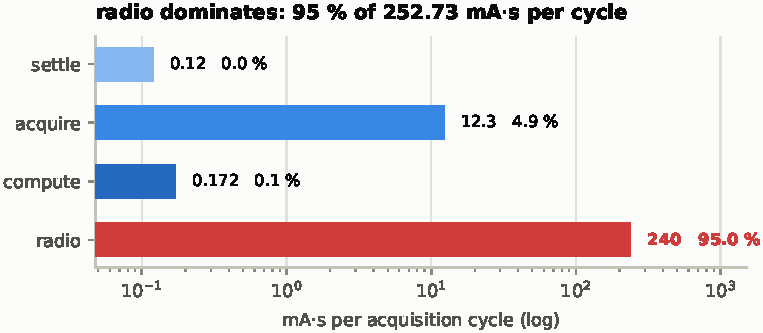
\includegraphics[width=0.66\linewidth]{kit_esp32s3_energy.pdf}
  \\[1.5mm]
  \begin{columns}[T]
    \begin{column}{0.46\textwidth}
      \scriptsize
      240 mA$\cdot$s per association --- \textbf{1\,400$\times$} the sensing and
      compute combined. Nothing about the DSP, the sensor or the record length
      changes that number.
      \\[1.5mm]
      So: 6-hour default interval, a 4096-frame queue, a transmit path that
      \emph{batches}, and deep sleep rather than light sleep (7 $\mu$A vs
      240 $\mu$A --- light sleep alone would be 40$\times$ the acquisition
      budget).
    \end{column}
    \begin{column}{0.5\textwidth}
      \scriptsize
      \textbf{The chain nobody expects:}
      \\[1mm]
      {\tiny\ttfamily
      Wi-Fi 350 mA peaks\\
      ~~-> rules out LiSOCl2 (pulse limit $\sim$10s of mA)\\
      ~~~~~-> must use Li-ion (2.5 \%/month = 72 uA)\\
      ~~~~~~~~-> self-discharge > circuit draw above 1 h\\
      ~~~~~~~~~~~-> life saturates near 2.7 years\\
      ~~~~~~~~~~~~~~-> honest answer: mains or PoE
      }
      \\[2mm]
      Compare the Nordic kit: LTE-M costs 95 mA$\cdot$s --- a \emph{more}
      expensive radio --- but its pulse profile permits a LiSOCl$_2$ D-cell at
      0.08 \%/month, giving \textbf{9.4 years}. Five times the life from the
      more expensive radio.
    \end{column}
  \end{columns}
\end{frame}

% ------------------------------------------------------------- dual core -----
\begin{frame}{Two things that are correctness requirements, not optimisations}
  \begin{columns}[T]
    \begin{column}{0.48\textwidth}
      \small\textbf{Dual-core}
      \\[1.5mm]
      \scriptsize
      \texttt{CONFIG\_FREERTOS\_UNICORE=n}, and not for throughput.
      \\[1mm]
      The ADXL355 FIFO is 96 samples --- \textbf{24 ms} at 4 kHz. The ESP-IDF
      Wi-Fi task outranks application tasks and can hold the CPU for tens of
      milliseconds during association.
      \\[1mm]
      On one core that overruns the FIFO, and the block becomes a concatenation
      of two different times: a spectrum with a step discontinuity that looks
      exactly like an impact train.
      \\[1mm]
      Three defences: acquisition pinned to core 1, the application never
      transmits during an acquisition, and the overrun flag refuses the block
      rather than repairing it.
    \end{column}
    \begin{column}{0.48\textwidth}
      \small\textbf{The sequence number in RTC memory}
      \\[1.5mm]
      \scriptsize
      Deep sleep restarts from \texttt{app\_main} with SRAM gone. Ingest
      deduplicates on \texttt{(device\_id, sequence)} so that store-and-forward
      replays are idempotent.
      \\[1mm]
      A node that restarts its counter at zero therefore has \textbf{every frame
      after the first wake silently discarded as a duplicate}. It looks healthy
      and transmits nothing --- the worst available failure mode, because it is
      invisible from both ends.
      \\[1mm]
      \texttt{pdm\_app\_restore\_sequence} was added to the shared core for
      exactly this, and the first-boot checklist in \texttt{tools/flash.sh} says
      to verify that the second wake emits sequence 1.
    \end{column}
  \end{columns}
\end{frame}

% ------------------------------------------------------------- the win -------
\begin{frame}{The kit's worst spec is also its best}
  \begin{columns}[T]
    \begin{column}{0.52\textwidth}
      \small
      The ADXL355's output rate comes from an internal oscillator with no
      tolerance better than \textbf{$\pm$5 \%} over temperature --- worse than
      the IIS3DWB's $\pm$3 \%.
      \\[2mm]
      \scriptsize
      But this board has a \textbf{$\pm$10 ppm crystal} and
      \texttt{esp\_timer}, so the true elapsed time of an acquisition is
      measurable to microseconds. \texttt{samples / elapsed} \emph{is} the real
      rate.
      \\[2mm]
      The STWIN.box cannot do this: its FIFO carries no timestamps at
      26.667 kHz and there is no reference clock path into the sensor. Its fix
      needs a reference tone through the self-test actuator.
    \end{column}
    \begin{column}{0.44\textwidth}
      \scriptsize
      \textbf{Why it matters.} A 3 \% rate error moves a 106 Hz BPFO line by
      3.2 Hz. By the fifth harmonic that is 16 Hz against a $\pm$10.6 Hz
      matching window, so the top harmonics fall outside and
      \texttt{n\_matched} under-reports exactly when the evidence is strongest.
      \\[2.5mm]
      \textbf{Status: identified, not implemented.}
      \texttt{pdm\_board\_acquire} reports the nominal rate with a comment
      saying so. It is the cheapest accuracy win anywhere in this repository and
      about a dozen lines of code.
    \end{column}
  \end{columns}
  \takeaway{The niche: brownfield retrofit, high asset count, a socket or PoE
    drop nearby. On battery, the ST and Nordic kits are better at their own jobs.}
\end{frame}

\end{document}
